\documentclass{article}

\usepackage{graphicx}
\usepackage{tikz}
\usepackage{tikzsymbols}
\usetikzlibrary{calc,patterns,shapes.geometric}
\pagestyle{empty}
\usepackage[margin=0pt]{geometry}
\geometry{papersize={14in,12in}}

\def\centerarc[#1](#2)(#3:#4:#5){\draw[#1] ($(#2)+({#5*cos(#3)},{#5*sin(#3)})$) arc (#3:#4:#5);}

\begin{document}
	\begin{figure}
		\centering
		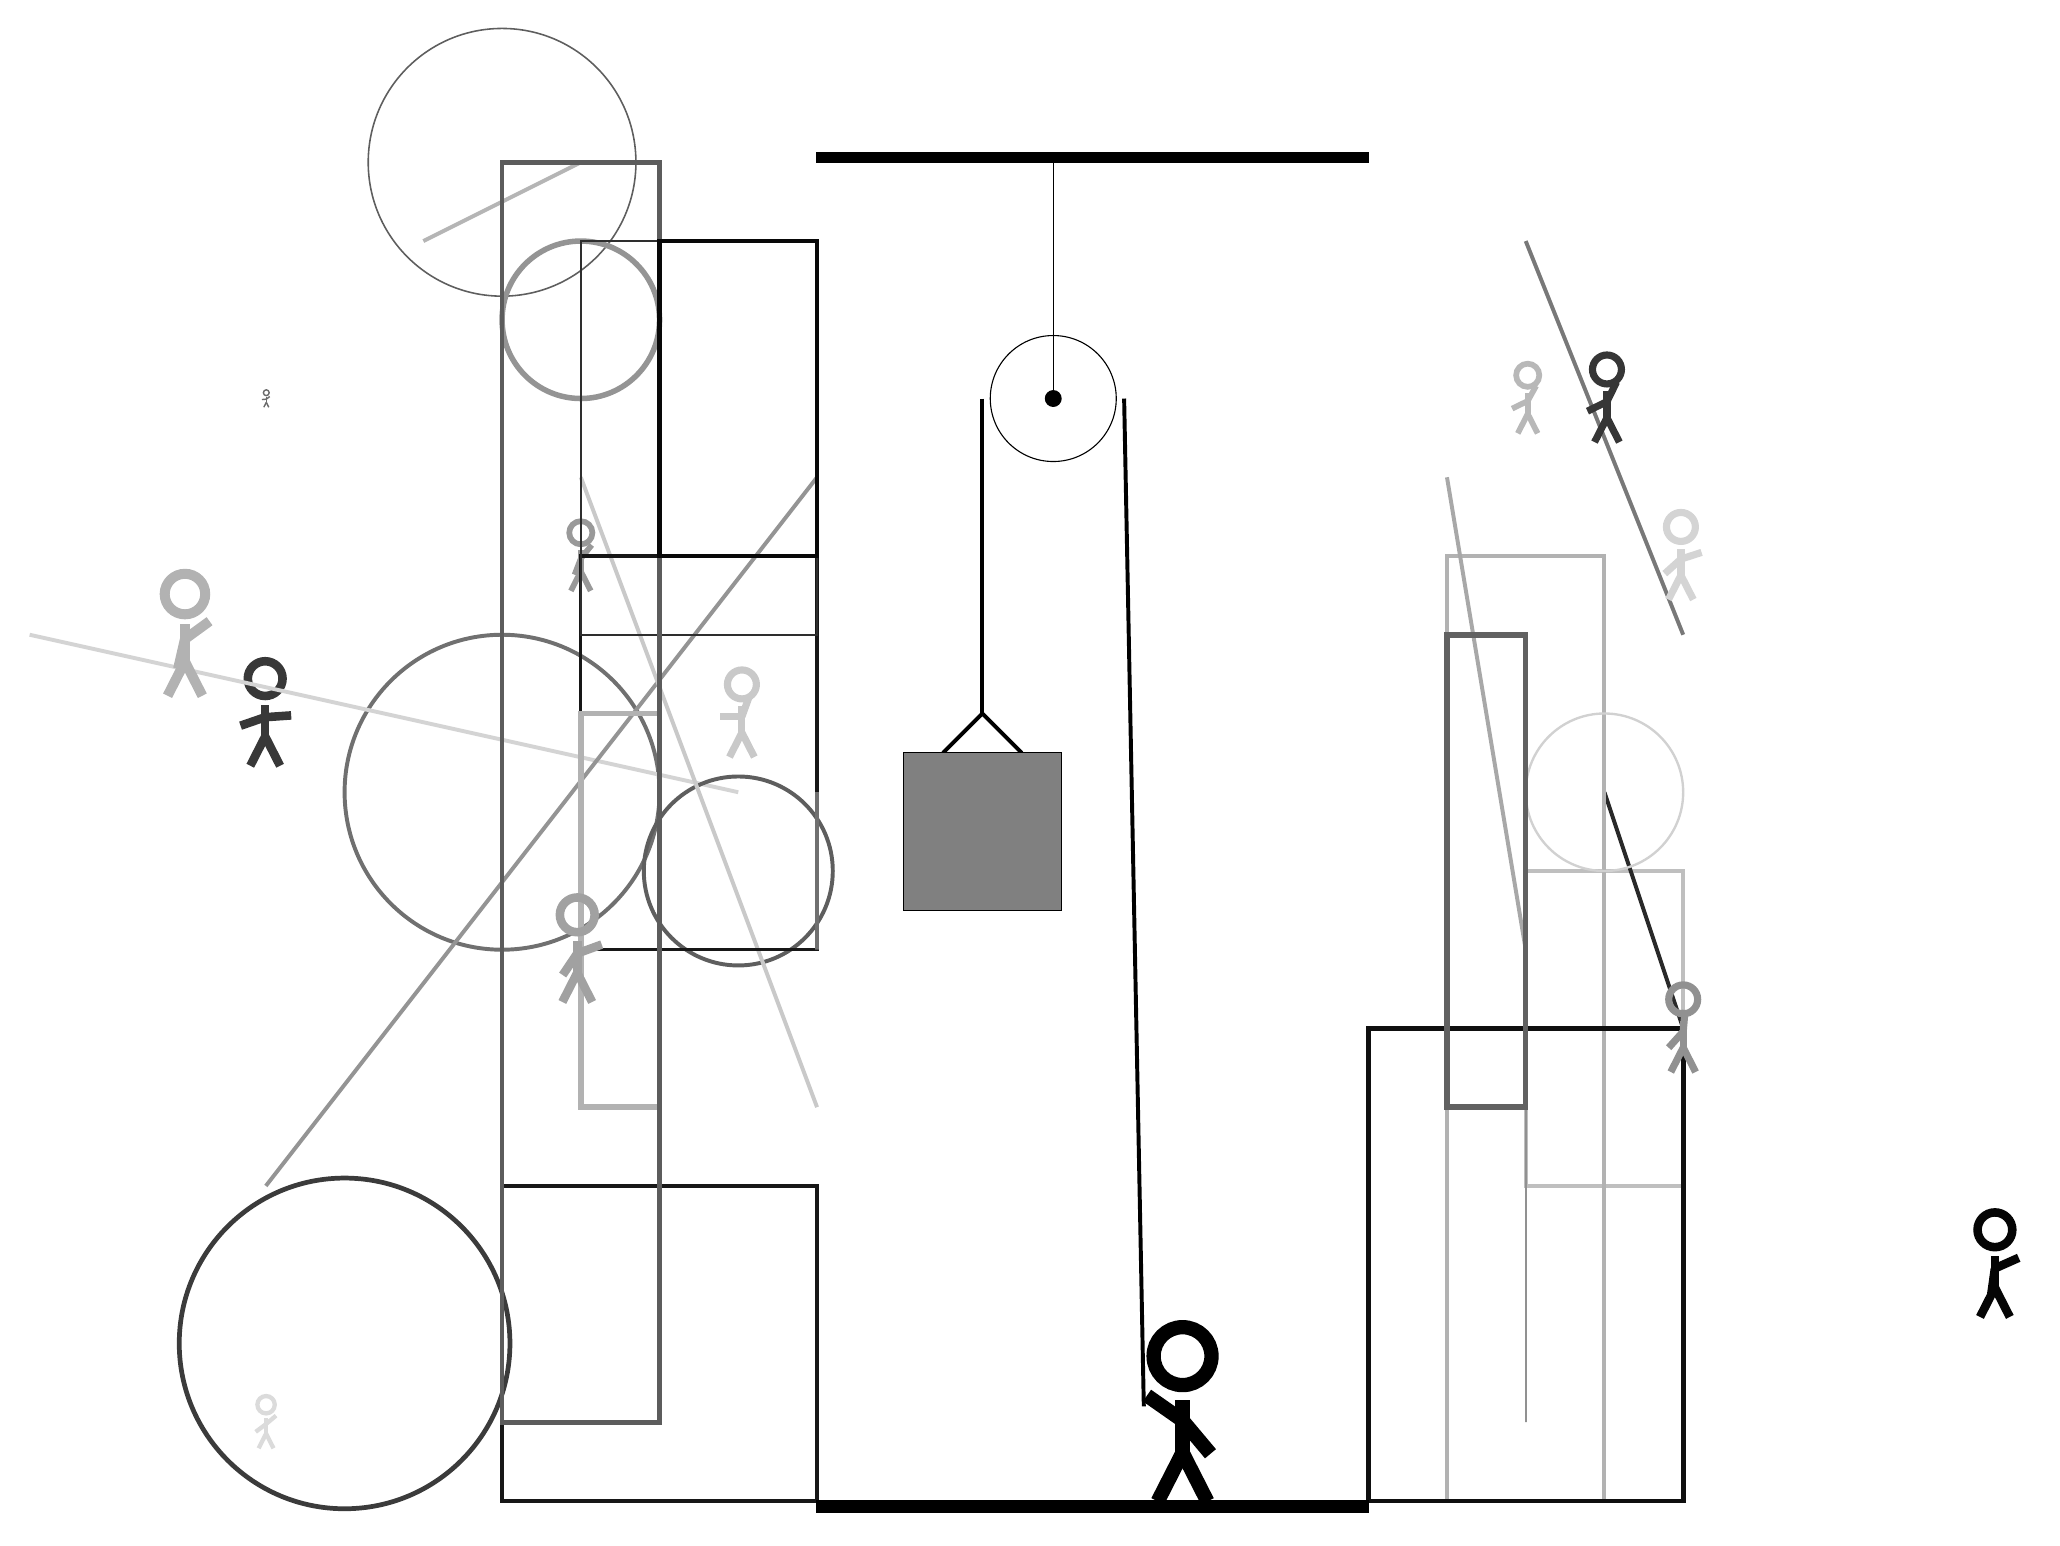
\begin{tikzpicture}
			%%%%% START %%%%%
			
			\draw[fill=black] (-2, 14) rectangle (5, 14.125);
			
			\node[line width=0.5mm, color=black!78] at (-9, 7) {\Strichmaxerl[6][19][4]};
			
			\draw[line width=0.5mm, color=black!25] (7, 5) rectangle (9, 1);
			\node[line width=0.7mm, color=black!40] at (-5, 9) {\Strichmaxerl[4][69][51]};
			\draw [line width=0.5mm, color=black!56](-6, 6) circle (2.0);
			\draw[line width=0.5mm, color=black!17](-3, 6) -- (-12, 8);
			
			\draw[line width=0.2mm, color=black!43] (7, 3) rectangle (7, -2);
			\node[line width=0.4mm, color=black!30] at (-10, 8) {\Strichmaxerl[7][77][36]};
			
			\draw [line width=0.2mm, color=black!63](-6, 14) circle (1.7);
			\draw[line width=0.5mm, color=black!84](8, 6) -- (9, 3);
			\draw [line width=0.5mm, color=black!63](-3, 5) circle (1.2);
			\node[line width=0.5mm, color=black!98] at (13, 0) {\Strichmaxerl[6][82][24]};
			\draw[line width=0.5mm, color=black!42](-2, 10) -- (-9, 1);
			\draw[line width=0.5mm, color=black!29](-7, 13) -- (-5, 14);
			
			\draw [line width=0.6mm, color=black!77](-8, -1) circle (2.1);
			\draw[line width=0.7mm, color=black!16] (7, 6) rectangle (7, 5);
			\draw[line width=0.5mm, color=black!21](-5, 10) -- (-2, 2);
			\draw[line width=0.4mm, color=black!91] (-2, 9) rectangle (-5, 4);
			\node[line width=0.4mm, color=black!14] at (-9, -2) {\Strichmaxerl[3][37][40]};
			\draw [line width=0.7mm, color=black!42](-5, 12) circle (1.0);
			\draw[line width=0.6mm, color=black!91] (-2, -3) rectangle (-6, 1);
			\draw[line width=0.5mm, color=black!30] (6, 9) rectangle (8, -3);
			
			\draw[line width=0.6mm, color=black!94] (5, -3) rectangle (9, 3);
			\draw[line width=0.3mm, color=black!82] (-2, 8) rectangle (-5, 13);
			\draw[line width=0.7mm, color=black!30] (-4, 2) rectangle (-5, 7);
			\draw[line width=0.6mm, color=black!64] (-4, -2) rectangle (-6, 14);
			
			\node[line width=0.7mm, color=black!21] at (-3, 7) {\Strichmaxerl[5][0][70]};
			
			\draw[line width=0.6mm, color=black!97] (-4, 9) rectangle (-2, 13);
			\draw[line width=0.5mm, color=black!34](6, 10) -- (7, 4);
			\node[line width=0.5mm, color=black!28] at (7, 11) {\Strichmaxerl[4][26][61]};
			\node[line width=0.2mm, color=black!58] at (-9, 11) {\Strichmaxerl[1][5][37]};
			\draw [line width=0.3mm, color=black!18](8, 6) circle (1.0);
			
			\draw[line width=0.6mm, color=black!56] (-2, 4) rectangle (-2, 6);
			\node[line width=0.7mm, color=black!43] at (9, 3) {\Strichmaxerl[5][48][85]};
			\draw[line width=0.5mm, color=black!53](7, 13) -- (9, 8);
			\node[line width=0.3mm, color=black!79] at (8, 11) {\Strichmaxerl[5][26][64]};
			\node[line width=0.7mm, color=black!17] at (9, 9) {\Strichmaxerl[5][42][18]};
			
			\node[line width=0.7mm, color=black!37] at (-5, 4) {\Strichmaxerl[6][56][20]};
			
			\draw[line width=0.7mm, color=black!62] (6, 2) rectangle (7, 8);
			
			\draw (1, 11) circle (0.8);
			\draw[fill=black] (1, 11) circle (0.1);
			\draw (1, 14) -- (1, 11);
			
			\draw[line width=0.5mm] (-0.4, 6.5) -- (0.1, 7.0) -- (0.6, 6.5);
			\draw[fill=black!50] (-0.9, 6.5) rectangle (1.1, 4.5);
			
			\draw[line width=0.5mm] (0.1, 11) -- (0.1, 7.0);
			\centerarc[line width=0.5mm](1, 11)(0:180:0.9);
			\draw[line width=0.5mm](1.9, 11) -- (2.15, -1.8);
			
			\node at (2.6, -1.9) {\Strichmaxerl[10][-35][-50]};
			
			\draw[fill=black] (-2, -3) rectangle (5, -3.15);
			
			%%%%% END %%%%%
		\end{tikzpicture}
	\end{figure}	
\end{document}